\documentclass{article}

\usepackage{arxiv}

\usepackage[utf8]{inputenc} % allow utf-8 input
\usepackage[T1]{fontenc}    % use 8-bit T1 fonts
\usepackage{lmodern}        % https://github.com/rstudio/rticles/issues/343
\usepackage{hyperref}       % hyperlinks
\usepackage{url}            % simple URL typesetting
\usepackage{booktabs}       % professional-quality tables
\usepackage{amsfonts}       % blackboard math symbols
\usepackage{nicefrac}       % compact symbols for 1/2, etc.
\usepackage{microtype}      % microtypography
\usepackage{graphicx}

\title{Unveiling Color Dynamics in Andy Warhol's ``Shot Marilyns'': A
Study on Visual Variations and Perception}

\author{
    Erick S. Arenas V
   \\
    Department of Statistics \\
    University of California, Davis \\
  Davis, CA 95616 \\
  \texttt{\href{mailto:esarenas@ucdavis.edu}{\nolinkurl{esarenas@ucdavis.edu}}} \\
   \And
    Weilin Cheng
   \\
    Department of Statistics \\
    University of California, Davis \\
  Davis, CA 95616 \\
  \texttt{\href{mailto:wncheng@ucdavis.edu}{\nolinkurl{wncheng@ucdavis.edu}}} \\
   \And
    Hengyuan Liu
   \\
    Department of Statistics \\
    University of California, Los Angeles \\
  Los Angeles, CA 90095 \\
  \texttt{\href{mailto:hengyuanliu@g.ucla.edu}{\nolinkurl{hengyuanliu@g.ucla.edu}}} \\
   \And
    Xinhui Luo
   \\
    Department of Statistics \\
    Tufts University \\
  Boston, MA 02155 \\
  \texttt{\href{mailto:xinhui.luo@tufts.edu}{\nolinkurl{xinhui.luo@tufts.edu}}} \\
   \And
    Kathy Mo
   \\
    Department of Statistics \\
    University of California, Los Angeles \\
  Los Angeles, CA 90095 \\
  \texttt{\href{mailto:kathymo24@g.ucla.edu}{\nolinkurl{kathymo24@g.ucla.edu}}} \\
   \And
    Li Yuan
   \\
    Department of Computer Science \\
    Swiss Federal Institute of Technology, Zurich \\
  8092 Zurich, Switzerland \\
  \texttt{\href{mailto:liyuan1@ethz.ch}{\nolinkurl{liyuan1@ethz.ch}}} \\
  }


% tightlist command for lists without linebreak
\providecommand{\tightlist}{%
  \setlength{\itemsep}{0pt}\setlength{\parskip}{0pt}}


% Pandoc citation processing
\newlength{\cslhangindent}
\setlength{\cslhangindent}{1.5em}
\newlength{\csllabelwidth}
\setlength{\csllabelwidth}{3em}
\newlength{\cslentryspacingunit} % times entry-spacing
\setlength{\cslentryspacingunit}{\parskip}
% for Pandoc 2.8 to 2.10.1
\newenvironment{cslreferences}%
  {}%
  {\par}
% For Pandoc 2.11+
\newenvironment{CSLReferences}[2] % #1 hanging-ident, #2 entry spacing
 {% don't indent paragraphs
  \setlength{\parindent}{0pt}
  % turn on hanging indent if param 1 is 1
  \ifodd #1
  \let\oldpar\par
  \def\par{\hangindent=\cslhangindent\oldpar}
  \fi
  % set entry spacing
  \setlength{\parskip}{#2\cslentryspacingunit}
 }%
 {}
\usepackage{calc}
\newcommand{\CSLBlock}[1]{#1\hfill\break}
\newcommand{\CSLLeftMargin}[1]{\parbox[t]{\csllabelwidth}{#1}}
\newcommand{\CSLRightInline}[1]{\parbox[t]{\linewidth - \csllabelwidth}{#1}\break}
\newcommand{\CSLIndent}[1]{\hspace{\cslhangindent}#1}

\usepackage{amsmath}
\usepackage{graphicx}
\usepackage{subcaption}
\usepackage{gensymb}
\begin{document}
\maketitle


\begin{abstract}
This study delves into the comparative analysis of five distinct
versions of Andy Warhol's ``Shot Marilyns,'' focusing on the intricacies
of their color composition and distribution. Employing a range of
analytical methods, including relative conditional entropy, this
research investigates the unique color distributions and interrelations
present in each artwork. Through the clustering of the artworks and the
meticulous examination of specified regions of interest (ROIs)---namely,
the backgrounds, hair, eyeshadow, and faces---we have unearthed profound
insights into the constructional variances and similarities among the
images. Our findings reveal that the presupposed uniformity in the
coloration of certain elements stands contradicted, thereby underscoring
the complexity and illusionary nature of color perception in visual art.
\end{abstract}

\keywords{
    shot marilyns
   \and
    marilyn monroe
   \and
    andy warhol
   \and
    region of interest
   \and
    python
  }

\hypertarget{introduction}{%
\section{Introduction}\label{introduction}}

In May 2022, one of Andy Warhol's ``Shot Marilyn'' portraits set a new
auction record, selling for \$195 million, as reported by the Los
Angeles Times. This unprecedented sale has renewed both public and
scholarly interest in Warhol's work, highlighting the enduring impact of
his art on contemporary culture. The ``Shot Marilyns'' series holds
immense value, not only monetarily but also in its profound impact on
contemporary art and its reflection of societal themes. The
record-breaking auction underscores its continued relevance and
fascination (Vankin 2022). Furthermore, Marilyn Monroe remains an iconic
figure whose image has permeated popular culture. Her tragic life story,
coupled with her enduring allure, makes her an intriguing subject for
artistic exploration (Gallery 2019). Warhol's unique art style,
characterized by his use of silkscreen printing and vibrant color
schemes, offers a rich field for visual analysis. His method of
mass-producing images and manipulating colors challenges traditional
notions of art and celebrity, making the ``Shot Marilyns'' series a
perfect case study for understanding his innovative approach (Lanchner
and Warhol 2008). Through this analysis, we aim to uncover new insights
into the interplay between celebrity, media, and art, enriching our
understanding of both Warhol's work and Monroe's legacy.

In 1964, amidst the bustling atmosphere of Andy Warhol's studio, The
Factory, a significant event led to the creation of the ``Shot
Marilyns'' series. Warhol, deeply influenced by Marilyn Monroe's tragic
death in 1962, began producing silkscreen portraits of her, capturing
the iconic actress's image through repetitive, vivid depictions
(Christie's 2022). The ``Shot Marilyns'' series features five portraits
shown in Figure \ref{fig:marilyn_variations}, each rendered in different
color schemes.

\begin{figure}[ht]
  \centering
  \begin{subfigure}{0.3\textwidth}
    \centering
    \includegraphics[width=125px]{main_files/figure-latex/1_1_orange_marilyn.jpg}
    \caption{Orange Marilyn}
    \label{fig:1_1_orange_marilyn}
  \end{subfigure}
  \hfill
  \begin{subfigure}{0.3\textwidth}
    \centering
    \includegraphics[width=125px]{main_files/figure-latex/1_2_red_marilyn.jpg}
    \caption{Red Marilyn}
    \label{fig:1_2_red_marilyn}
  \end{subfigure}
  \hfill
  \begin{subfigure}{0.3\textwidth}
    \centering
    \includegraphics[width=125px]{main_files/figure-latex/1_3_turq_marilyn.jpg}
    \caption{Turquoise Marilyn}
    \label{fig:1_3_turq_marilyn}
  \end{subfigure}

  \vspace{1em}

  \begin{minipage}{0.6\textwidth}
    \centering
    \begin{subfigure}{0.45\textwidth}
      \centering
      \includegraphics[width=125px]{main_files/figure-latex/1_4_blue_marilyn.jpg}
      \caption{Blue Marilyn}
      \label{fig:1_4_blue_marilyn}
    \end{subfigure}
    \hfill
    \begin{subfigure}{0.45\textwidth}
      \centering
      \includegraphics[width=125px]{main_files/figure-latex/1_5_eggblue_marilyn.jpg}
      \caption{Eggblue Marilyn}
      \label{fig:1_5_eggblue_marilyn}
    \end{subfigure}
  \end{minipage}

  \caption{The five portraits in Andy Warhol's "Shot Marilyns" series, each showcasing Marilyn Monroe in distinct color schemes: (a) Orange Marilyn, (b) Red Marilyn, (c) Turquoise Marilyn, (d) Blue Marilyn, and (e) Eggblue Marilyn. These variations exemplify Warhol's innovative use of color and his unique approach to portraiture. Image source: The Interior Review. Retrieved from https://www.theinteriorreview.com/story/2022/5/10/critically-assessing-warhols-shot-sage-blue-marilyn.}
  \label{fig:marilyn_variations}
\end{figure}

The name ``Shot Marilyns'' originates from an incident involving Dorothy
Podber, a performance artist and frequent visitor to The Factory. One
day, Podber, accompanied by Warhol's friend and photographer Bill Name,
observed the Marilyn portraits lined up against a wall. She asked Warhol
for permission to ``shoot'' them, which Warhol, interpreting it as a
request to photograph the artworks, granted. Unexpectedly, Podber pulled
out a revolver and fired a shot, piercing four of the five canvases
through the forehead (Ghighi 2022). This act of violence not only
created physical damage but also added a layer of historical intrigue
and controversy to Warhol's work, further embedding it into the fabric
of pop culture and art history.

In this paper, we aim to conduct a comprehensive analysis of Andy
Warhol's ``Shot Marilyns'' series using several advanced techniques.
First, we will analyze the relative conditional entropy of the pixel
color distribution in RGB (red, green, blue) space to understand the
variations in color across the different portraits. This will provide
insights into the underlying patterns and complexity of Warhol's use of
color. Next, we will create 3D scatter plots to visualize how each pixel
color is distributed in the RGB space, enabling us to observe the
distinct color palettes used in each image. We will also apply K-means
cluster analysis to identify and compare the primary color clusters
within the portraits, highlighting different regions of interest (ROI)
such as the background, hair, eyeshadow, and face. Additionally, we will
focus on digitally repairing the ``Blue Marilyn'' using K-Nearest
Neighbors to model and analyze the RGB distribution around the
gunshot-damaged area. This restoration will involve capturing the
gunshot region and using color distribution data to reconstruct the
damaged section, preserving the artwork's integrity. Through these
methods, we aim to gain a deeper understanding of Warhol's artistic
techniques and the visual impact of his ``Shot Marilyns'' series. While
our analysis strives for objectivity, we acknowledge that
interpretations of art can be inherently subjective.

\hypertarget{methods}{%
\section{Methods}\label{methods}}

An image is composed of pixels, each containing three color components:
Red (R), Green (G), and Blue (B), denoted as (R, G, B) respectively.
These components determine the intensity of their respective colors,
with each component represented by an integer value within the range of
0 to 255 in the RGB color space. Therefore, each color component is a
discrete variable capable of assuming 256 distinct values. In the
equations below, \(Y=y\) or \(X=x\) can be selected from any of the
three color components, R, G, or B. For this study, each image in the
``Shot Marilyns'' series has a resolution of 960 by 960 pixels.

\hypertarget{entropy-calculation}{%
\subsection{Entropy Calculation}\label{entropy-calculation}}

The probability of a specific color component, \(P(Y=y)\), is determined
by dividing the number of pixels with color coordinates corresponding to
that component by the total number of color components in the entire
image. The following equations illustrate the calculation of entropy,
conditional entropy, and relative conditional entropy introduced by
Shannon (1948).

The entropy of a color component \(Y\) is defined as:

\begin{equation}
  H(Y) = - \sum_{y=0}^{255} P(Y = y) \cdot \log(P(Y = y))
\end{equation}

The conditional entropy of \(Y\) given \(X\) is given by:

\begin{equation}
  H(Y|X) = \sum_{x=0}^{255} P(X = x) \cdot H(Y|X = x) = - \sum_{x=0}^{255} \sum_{y=0}^{255} P(X = x, Y = y) \log_2 \left(\frac{P(X = x, Y = y)}{P(X = x)}\right)
\end{equation}

The relative conditional entropy is calculated using the following
formula:

\begin{equation}
  HR(X|Y) = \frac{H(X|Y)}{H(X)}
\end{equation}

\hypertarget{k-means-clustering-analysis}{%
\subsection{K-Means Clustering
Analysis}\label{k-means-clustering-analysis}}

In the clustering analysis, we applied K-Means clustering to examine the
color dynamics in Andy Warhol's ``Shot Marilyns'' series. For each
image, we specified 15 clusters and used the ``k-means++''
initialization method. This initialization method, introduced by Arthur
and Vassilvitskii (2007), improves the convergence speed and accuracy of
the K-Means algorithm by spreading out the initial cluster centers. This
method is particularly effective in avoiding poor clustering results due
to the random placement of initial centroids.

Mathematically, the K-Means algorithm minimizes the following objective
function:

\begin{equation}
  J = \sum_{i=1}^{k} \sum_{x \in C_i} \| x - \mu_i \|^2
\end{equation}

where \(k\) is the number of clusters, \(C_i\) is the set of points
belonging to cluster \(i\), \(x\) represents a data point, and \(\mu_i\)
is the centroid of cluster \(i\). The ``k-means++'' algorithm
initializes the centroids by first selecting one random data point as
the first centroid. Subsequent centroids are chosen based on a
probability proportional to the squared distance from the nearest
existing centroid. This process can be expressed as:

\begin{equation}
  P(x) = \frac{D(x)^2}{\sum_{x' \in X} D(x')^2}
\end{equation}

where \(D(x)\) is the distance from the point \(x\) to the nearest
centroid already chosen.

Using this method, we applied K-Means clustering to the entire images
and specific regions of interest (ROI) in each image. The clustering
algorithm grouped pixels into clusters based on their RGB values,
effectively identifying the predominant colors in each image. This
approach allowed us to quantify and visualize the distribution of
colors, revealing the underlying color patterns and variations within
the artworks. The resulting clusters were then analyzed to understand
the prominence of specific colors across the series, as depicted in the
corresponding bar charts and ribbon visualizations. These visualizations
highlight the distinctive color schemes employed by Warhol, providing
insights into his artistic technique and color usage.

\hypertarget{roi-extraction}{%
\subsection{ROI Extraction}\label{roi-extraction}}

In our Region of Interest (ROI) analysis, we targeted specific segments
of the images such as the background, hair, eye shadows, and face. We
began by converting the images to the HSV color space using OpenCV's
conversion functions, which facilitate more effective identification and
segmentation of specific color ranges. By manually determining the
minimum and maximum HSV values within selected regions, we created color
masks using OpenCV's masking functions to isolate these target areas.
These masks highlighted the pixels that fell within the specified HSV
range, effectively isolating the desired colors from the rest of the
image. Once the masks were applied, we used image processing techniques
to extract only the parts of the image that matched the mask, discarding
the rest. This allowed us to focus on the color features of interest.
The resultant ROIs were then processed and saved for detailed analysis.
This method, enhanced by the precise capabilities of OpenCV and guided
by best practices from Culjak et al. (2012), enabled us to highlight
specific color features in Warhol's artwork, providing nuanced insights
into his use of color and its variations, and ensuring accurate and
efficient color segmentation and analysis.

\hypertarget{k-nearest-neighbors-repair}{%
\subsection{K-Nearest Neighbors
Repair}\label{k-nearest-neighbors-repair}}

To address the damaged sections of the ``Blue Marilyn'' image, we
employed K-Nearest Neighbors (KNN) regression for image repair. This
method involves identifying the coordinates of the damaged pixels and
using the surrounding undamaged pixels to predict their values. The KNN
regression model, with a specified number of neighbors, was trained on
the undamaged pixels' RGB values. The model then predicted the RGB
values for the damaged pixels, effectively restoring the affected area.
This approach allowed us to maintain the image's visual consistency by
leveraging the spatial color information of the undamaged regions. The
repaired images were subsequently saved and analyzed to ensure the
accuracy and aesthetic integrity of the restoration process.

\hypertarget{data-description}{%
\section{Data Description}\label{data-description}}

Our study utilized a dataset comprising five images titled Orange
Marilyn, Red Marilyn, Turquoise Marilyn, Blue Marilyn, and Eggblue
Marilyn. These images are digitally encoded in the RGB color channels,
which synthesize a spectrum of colors through the additive mixing of
Red, Green, and Blue lights. To enhance future data visualizations, we
also converted the RGB values into Hexadecimal representations. Each
image measures 960 by 960 pixels, resulting in 921,600 unique data
points per image, each specified by a distinct location and chromatic
composition. In this additive color model, the intensity of each primary
color (Red, Green, and Blue) is quantized into discrete levels ranging
from 0 to 255, providing a finite palette within this cubic color space.
Each pixel's color is quantified based on the RGB values, making it part
of a discrete color space where the combination of these three channels
can reproduce a wide array of colors.

\begin{figure}[ht]
  \centering
  \begin{subfigure}{0.3\textwidth}
    \centering
    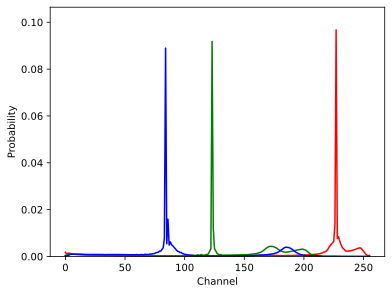
\includegraphics[width=125px]{main_files/figure-latex/2_1_orange_marilyn_dist.pdf}
    \caption{Orange Marilyn}
    \label{fig:2_1_orange_marilyn_dist}
  \end{subfigure}
  \hfill
  \begin{subfigure}{0.3\textwidth}
    \centering
    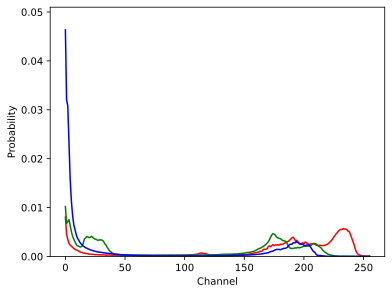
\includegraphics[width=125px]{main_files/figure-latex/2_2_red_marilyn_dist.pdf}
    \caption{Red Marilyn}
    \label{fig:2_2_red_marilyn_dist}
  \end{subfigure}
  \hfill
  \begin{subfigure}{0.3\textwidth}
    \centering
    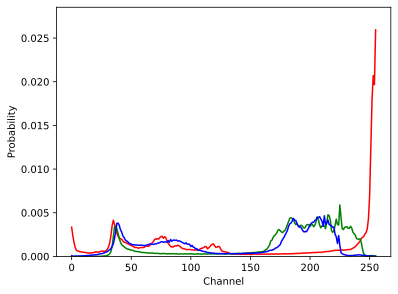
\includegraphics[width=125px]{main_files/figure-latex/2_3_turq_marilyn_dist.pdf}
    \caption{Turquoise Marilyn}
    \label{fig:2_3_turq_marilyn_dist}
  \end{subfigure}

  \vspace{1em}

  \begin{minipage}{0.6\textwidth}
    \centering
    \begin{subfigure}{0.45\textwidth}
      \centering
      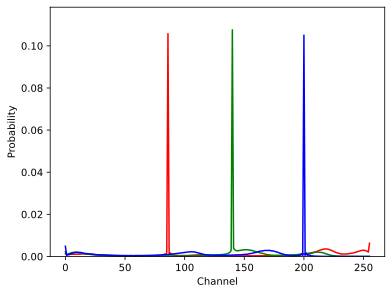
\includegraphics[width=125px]{main_files/figure-latex/2_4_blue_marilyn_dist.pdf}
      \caption{Blue Marilyn}
      \label{fig:2_4_blue_marilyn_dist}
    \end{subfigure}
    \hfill
    \begin{subfigure}{0.45\textwidth}
      \centering
      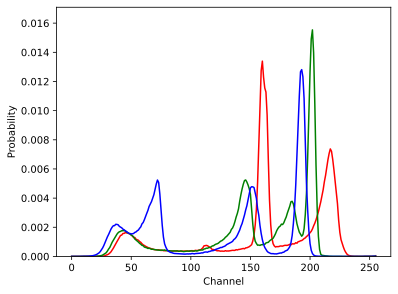
\includegraphics[width=125px]{main_files/figure-latex/2_5_eggblue_marilyn_dist.pdf}
      \caption{Eggblue Marilyn}
      \label{fig:2_5_eggblue_marilyn_dist}
    \end{subfigure}
  \end{minipage}

  \caption{Distributions of values of Red, Green, and Blue channels for five images with all pixels}
  \label{fig:marilyn_dist}
\end{figure}

Our initial analysis involved examining the distribution profiles of the
RGB channels in the images. Figure 2 illustrates the variations in the
red, green, and blue distributions across the five images. Notably,
images (a) and (d) exhibit significant differences compared to the
others.

In the Orange Marilyn image (a), the blue channel's highest probability
density is localized within the {[}50, 100{]} range, reaching
approximately 8.5\%. The green channel peaks between {[}120, 130{]} with
a probability around 9\%. Additionally, the blue channel shows another
notable concentration in the {[}220, 240{]} range, with a likelihood of
about 10\%.

Interestingly, the green channel probabilities in image (d) closely
mirror those in image (a), predominantly in the {[}120, 130{]} range.
However, image (d) differs significantly in the red and blue spectra.
The red channel in image (d) peaks in the {[}70, 80{]} range with an
11\% likelihood, while the blue channel's highest probability is within
the {[}190, 210{]} range, also accounting for an 11\% probability. These
differences in the red and blue channel distributions between images (d)
and (a) highlight their unique color distribution attributes.

Images (b) Red Marilyn and (c) Turquoise Marilyn display highly skewed
patterns. Image (b) shows a right-skewed distribution with the blue
channel having the highest probability around 0.05, while the red and
green channels are not as distinctive. In contrast, image (c) is
left-skewed, with the red channel showing the highest probability around
0.025. Both images exhibit less distinct differences between the red,
green, and blue distributions.

The Eggblue Marilyn image (e) presents a harmonious entanglement of the
red, blue, and green channels. Each channel has a relatively similar
probability distribution, with no single color dominating significantly.
The red, blue, and green channels each have their highest probabilities
around 0.015, indicating a balanced color distribution across the image.

This analysis reveals the diverse color distribution patterns in
Warhol's ``Shot Marilyns,'' highlighting the unique attributes and
artistic techniques employed in each painting.

\begin{figure}[ht]
  \centering
  \begin{subfigure}{0.3\textwidth}
    \centering
    \includegraphics[width=125px]{main_files/figure-latex/3_1_orange_marilyn_entropy.pdf}
    \caption{Orange Marilyn Relative Conditional Entropy}
    \label{fig:3_1_orange_marilyn_entropy}
  \end{subfigure}
  \hfill
  \begin{subfigure}{0.3\textwidth}
    \centering
    \includegraphics[width=125px]{main_files/figure-latex/3_2_red_marilyn_entropy.pdf}
    \caption{Red Marilyn Relative Conditional Entropy}
    \label{fig:3_2_red_marilyn_entropy}
  \end{subfigure}
  \hfill
  \begin{subfigure}{0.3\textwidth}
    \centering
    \includegraphics[width=125px]{main_files/figure-latex/3_3_turq_marilyn_entropy.pdf}
    \caption{Turquoise Marilyn Relative Conditional Entropy}
    \label{fig:3_3_turq_marilyn_entropy}
  \end{subfigure}

  \vspace{1em} % Add some vertical space between rows

  \begin{minipage}{0.6\textwidth}
    \centering
    \begin{subfigure}{0.45\textwidth}
      \centering
      \includegraphics[width=125px]{main_files/figure-latex/3_4_blue_marilyn_entropy.pdf}
      \caption{Blue Marilyn Relative Conditional Entropy}
      \label{fig:3_4_blue_marilyn_entropy}
    \end{subfigure}
    \hfill
    \begin{subfigure}{0.45\textwidth}
      \centering
      \includegraphics[width=125px]{main_files/figure-latex/3_5_eggblue_marilyn_entropy.pdf}
      \caption{Eggblue Marilyn Relative Conditional Entropy}
      \label{fig:3_5_eggblue_marilyn_entropy}
    \end{subfigure}
  \end{minipage}

  \caption{The relative conditional entropy values among the red, green, and blue coordinates of pixels}
  \label{fig:marilyn_entropy}
\end{figure}

After analyzing the RGB distribution of each image, we further
investigated the relationship between pairs of primary colors in the
five images by calculating their relative conditional entropy (HR) (see
Methods 2.1). This metric quantifies the shared information or
dependency between two color channels, with lower HR values indicating
stronger dependencies and higher values suggesting greater independence.
HR ranges from 0 to 1, where 0 signifies complete dependency and 1
represents total independence.

Figure 3 presents the HR values for nine color pairs in each of the five
images: Orange Marilyn, Red Marilyn, Turquoise Marilyn, Blue Marilyn,
and Eggblue Marilyn. As expected, comparing a color to itself yields a
conditional entropy of zero. High HR values for different color pairs
indicate minimal dependency between them.

In the Orange Marilyn image (a), the HR values are relatively high
between different color pairs, with the blue and red channels showing an
HR value of 0.669, indicating a moderate level of independence.

In the Red Marilyn image (b), all the pairs has higher HR values compare
to the other images which indicated red, blue, and green colors high
independence each other. Notably, the HR value for the red channel
relative to the blue channel is 0.874, signifying very strong
independence between these two channels.

For the Turquoise Marilyn image (c), the HR values also reflect notable
independence between color pairs. The HR value between the red and blue
channels is 0.757, and between the blue and green channels, it is 0.673,
indicating a significant level of independence among the color channels.

The Blue Marilyn image (d) exhibits moderate HR values between the color
pairs. The red and blue channels showing an HR value of 0.605 and the
green and blue channels at 0.546. This suggests a balanced dependency
among the color channels in other images.

Finally, the Eggblue Marilyn image (e) shows harmonious HR values among
the color pairs, with the red and blue channels having an HR value of
0.663 and the green and blue channels at 0.572. These values indicate a
moderate level of independence among the color channels.

Overall, these HR values highlight the unique color relationships and
dependencies within each of Warhol's ``Shot Marilyns'' paintings,
providing insights into his use of color to create depth and visual
interest.

\hypertarget{data-exploration-and-visualization-analysis}{%
\section{Data Exploration and Visualization
Analysis}\label{data-exploration-and-visualization-analysis}}

The figures below display the RGB space occupied by the pixels of
various Marilyn paintings from four different angles. Each subplot
reveals the distribution and density of pixel colors in the 3D RGB color
space, providing insights into the color composition and variations
within the images.

\begin{figure}[ht]
  \centering
  \begin{subfigure}{0.45\textwidth}
    \includegraphics[width=\textwidth]{main_files/figure-latex/4_1_orange_marilyn_original_scatter.jpg}
    \caption{Orange Marilyn RGB Space}
    \label{fig:4_1_orange_marilyn_original_scatter}
  \end{subfigure}
  \hfill
  \begin{subfigure}{0.45\textwidth}
    \includegraphics[width=\textwidth]{main_files/figure-latex/4_2_orange_marilyn_original_scatter.jpg}
    \caption{Orange Marilyn RGB Space}
    \label{fig:4_2_orange_marilyn_original_scatter}
  \end{subfigure}
  \label{fig:orange_marilyn_original_scatter_1}
\end{figure}

\begin{figure}[ht]\ContinuedFloat
  \centering
  \begin{subfigure}{0.45\textwidth}
    \includegraphics[width=\textwidth]{main_files/figure-latex/4_3_orange_marilyn_original_scatter.jpg}
    \caption{Orange Marilyn RGB Space}
    \label{fig:4_3_orange_marilyn_original_scatter}
  \end{subfigure}
  \hfill
  \begin{subfigure}{0.45\textwidth}
    \includegraphics[width=\textwidth]{main_files/figure-latex/4_4_orange_marilyn_original_scatter.jpg}
    \caption{Orange Marilyn RGB Space }
    \label{fig:4_4_orange_marilyn_original_scatter}
  \end{subfigure}
  \caption{The RGB space occupied by the pixels for the entire image of Orange Marilyn, showing different angles: (a) 30 \degree elevation, 45 \degree azimuth, (b) 30 \degree elevation, 135 \degree azimuth, (c) 30 \degree elevation, 225 \degree azimuth, (d) 30 \degree elevation, 315 \degree azimuth. These variations highlight the color distribution within the artwork.}
  \label{fig:orange_marilyn_original_scatter_2}
\end{figure}

Figure 4 displays the RGB space of ``Orange Marilyn'' from four
different angles. In (a), the density of pixels representing the
background part of the image is shown, revealing a balanced mix of
colors including orange, yellow, pink, red, and blue. These colors
reflect the different dominant areas of the painting: the orange
background, yellow hair, pink face, red lips, and blue eye shades. The
shape of the 3D scatter plot in (a) indicates a broad, dispersed
distribution of colors, showing the diverse color use in the background
and facial features.

In (b), the plot illustrates how colors are distributed from darker
pixels at the bottom to brighter pixels at the top, highlighting shading
gradients. This gradient reflects the shading around Marilyn's facial
features and hair, adding depth to the portrait. The darker pixels
likely represent shadows in the hair and facial contours, while the
brighter pixels correspond to highlights on her face and hair.

In (c), the concentration of the brightest pixels is evident, showing
specific groupings likely related to prominent features. This highlights
the intense colors used in Marilyn's lips, eyes, and other facial
highlights. The plot suggests a focused clustering of bright colors,
indicating areas where Warhol applied more vivid hues to draw attention.

In (d), the color distribution from dark to light is presented from a
different angle, allowing us to observe the distribution of colors in
areas such as hair and eye shades with less red. This provides a
different perspective on the artwork's color dynamics, showing how the
turquoise and yellow shades in the hair and the blue in the eyes are
distributed. The shapes in (b) through (d) all reflect a similar
elongated form, resembling a long funnel, showing a clear gradient from
dark to light colors. This consistent shape across different angles
highlights the structured way Warhol applied color to create depth and
contrast in the ``Orange Marilyn'' painting.

\begin{figure}[ht]
  \centering
  \begin{subfigure}{0.45\textwidth}
    \includegraphics[width=\textwidth]{main_files/figure-latex/4_5_red_marilyn_original_scatter.jpg}
    \caption{Red Marilyn RGB Space}
    \label{fig:4_5_red_marilyn_original_scatter}
  \end{subfigure}
  \hfill
  \begin{subfigure}{0.45\textwidth}
    \includegraphics[width=\textwidth]{main_files/figure-latex/4_6_red_marilyn_original_scatter.jpg}
    \caption{Red Marilyn RGB Space}
    \label{fig:4_6_red_marilyn_original_scatter}
  \end{subfigure}
  \label{fig:red_marilyn_original_scatter_1}
\end{figure}

\begin{figure}[ht]\ContinuedFloat
  \centering
  \begin{subfigure}{0.45\textwidth}
    \includegraphics[width=\textwidth]{main_files/figure-latex/4_7_red_marilyn_original_scatter.jpg}
    \caption{Red Marilyn RGB Space}
    \label{fig:4_7_red_marilyn_original_scatter}
  \end{subfigure}
  \hfill
  \begin{subfigure}{0.45\textwidth}
    \includegraphics[width=\textwidth]{main_files/figure-latex/4_8_red_marilyn_original_scatter.jpg}
    \caption{Red Marilyn RGB Space}
    \label{fig:4_8_red_marilyn_original_scatter}
  \end{subfigure}
  \caption{The RGB space occupied by the pixels for the entire image of Red Marilyn, showing different angles: (a) 30 \degree elevation, 45 \degree azimuth, (b) 30 \degree elevation, 135 \degree azimuth, (c) 30 \degree elevation, 225 \degree azimuth, (d) 30 \degree elevation, 315 \degree azimuth. These variations highlight the color distribution within the artwork.}
  \label{fig:red_marilyn_original_scatter_2}
\end{figure}

Figure 5 displays the RGB space of ``Red Marilyn'' from four different
angles. The red color represents the background of the portrait. The
yellow color of Marilyn's hair is brighter than ``Orange Marilyn,''
along with her eye shadow and clothes.

In (a), the colors and shape of the figure is similar to the
corresponding image for ``Orange Marilyn.'' However, there is a much
larger prominence of orange, creating a concave shape at the lower left.
The longer stretches of yellow and blue correspond to the brighter
shades of these colors in this portrait, compared to ``Orange Marilyn.''

The shapes in (b) through (d) all reflect a similar elongated form as
seen in ``Orange Marilyn,'' but with a more spread-out appearance,
resembling a long and thick funnel. This shape shows a clear gradient
from dark to light colors, indicating that the colors are brighter,
bolder, and more impactful than in ``Orange Marilyn.'' This consistent
shape across different angles highlights the structured way Warhol
applied color to create depth and contrast in the ``Red Marilyn''
painting.

\begin{figure}[ht]
  \centering
  \begin{subfigure}{0.45\textwidth}
    \includegraphics[width=\textwidth]{main_files/figure-latex/4_9_turq_marilyn_original_scatter.jpg}
    \caption{Turquoise Marilyn RGB Space}
    \label{fig:4_9_turq_marilyn_original_scatter}
  \end{subfigure}
  \hfill
  \begin{subfigure}{0.45\textwidth}
    \includegraphics[width=\textwidth]{main_files/figure-latex/4_10_turq_marilyn_original_scatter.jpg}
    \caption{Turquoise Marilyn RGB Space}
    \label{fig:4_10_turq_marilyn_original_scatter}
  \end{subfigure}
  \label{fig:turq_marilyn_original_scatter_1}
\end{figure}

\begin{figure}[ht]\ContinuedFloat
  \centering
  \begin{subfigure}{0.45\textwidth}
    \includegraphics[width=\textwidth]{main_files/figure-latex/4_11_turq_marilyn_original_scatter.jpg}
    \caption{Turquoise Marilyn RGB Space}
    \label{fig:4_11_turq_marilyn_original_scatter}
  \end{subfigure}
  \hfill
  \begin{subfigure}{0.45\textwidth}
    \includegraphics[width=\textwidth]{main_files/figure-latex/4_12_turq_marilyn_original_scatter.jpg}
    \caption{Turquoise Marilyn RGB Space}
    \label{fig:4_12_turq_marilyn_original_scatter}
  \end{subfigure}
  \caption{The RGB space occupied by the pixels for the entire image of Turquoise Marilyn, showing different angles: (a) 30 \degree elevation, 45 \degree azimuth, (b) 30 \degree elevation, 135 \degree azimuth, (c) 30 \degree elevation, 225 \degree azimuth, (d) 30 \degree elevation, 315 \degree azimuth. These variations highlight the color distribution within the artwork.}
  \label{fig:turq_marilyn_original_scatter_2}
\end{figure}

Figure 6 displays the RGB space of ``Turquoise Marilyn'' from four
different angles. The turquoise color represents the background. The
color of Marilyn's hair, skin, and eye shadow are the brightest of all
five portraits. There is also a distinct lack of color to the right of
her neck. This is all showcased in the RGB space.

Unlike the previous two portraits, the shape image (a) for ``Turquoise
Marilyn'' lacks a prominent amount of orange color, creating an upside
down ``V'' shape.

Image (b) through (d) are similar to the previous ``Shot Marilyn's,''
just with lighter shades of color. The wide shapes for each one resemble
``Red Marilyn.''

The shapes in (a) through (d) reflect a similar elongated form,
resembling a long and wide funnel, showing a clear gradient from dark to
light colors. This highlights how the colors are brighter in ``Turquoise
Marilyn,'' emphasizing the structured application of color by Warhol to
create depth and contrast.

\begin{figure}[ht]
  \centering
  \begin{subfigure}{0.45\textwidth}
    \includegraphics[width=\textwidth]{main_files/figure-latex/4_13_blue_marilyn_original_scatter.jpg}
    \caption{Blue Marilyn RGB Space}
    \label{fig:4_13_blue_marilyn_original_scatter}
  \end{subfigure}
  \hfill
  \begin{subfigure}{0.45\textwidth}
    \includegraphics[width=\textwidth]{main_files/figure-latex/4_14_blue_marilyn_original_scatter.jpg}
    \caption{Blue Marilyn RGB Space}
    \label{fig:4_14_blue_marilyn_original_scatter}
  \end{subfigure}
  \label{fig:blue_marilyn_original_scatter_1}
\end{figure}

\begin{figure}[ht]\ContinuedFloat
  \centering
  \begin{subfigure}{0.45\textwidth}
    \includegraphics[width=\textwidth]{main_files/figure-latex/4_15_blue_marilyn_original_scatter.jpg}
    \caption{Blue Marilyn RGB Space}
    \label{fig:4_15_blue_marilyn_original_scatter}
  \end{subfigure}
  \hfill
  \begin{subfigure}{0.45\textwidth}
    \includegraphics[width=\textwidth]{main_files/figure-latex/4_16_blue_marilyn_original_scatter.jpg}
    \caption{Blue Marilyn RGB Space}
    \label{fig:4_16_blue_marilyn_original_scatter}
  \end{subfigure}
  \caption{The RGB space occupied by the pixels for the entire image of Blue Marilyn, showing different angles: (a) 30 \degree elevation, 45 \degree azimuth, (b) 30 \degree elevation, 135 \degree azimuth, (c) 30 \degree elevation, 225 \degree azimuth, (d) 30 \degree elevation, 315 \degree azimuth. These variations highlight the color distribution within the artwork.}
  \label{fig:blue_marilyn_original_scatter_2}
\end{figure}

Figure 7 displays the RGB space of ``Blue Marilyn'' from four different
angles. The blue represents the background of the portrait. The colors
representing Marilyn's hair and skin are darker than all of the previous
portraits. The smaller shapes in image (a) through (d) are similar to
``Orange Marilyn.'' The colors in each RGB space are less spread out,
while the shades of color themselves are darker than the previous
portraits.

\begin{figure}[ht]
  \centering
  \begin{subfigure}{0.45\textwidth}
    \includegraphics[width=\textwidth]{main_files/figure-latex/4_17_eggblue_marilyn_original_scatter.jpg}
    \caption{Eggblue Marilyn RGB Space}
    \label{fig:4_17_eggblue_marilyn_original_scatter}
  \end{subfigure}
  \hfill
  \begin{subfigure}{0.45\textwidth}
    \includegraphics[width=\textwidth]{main_files/figure-latex/4_18_eggblue_marilyn_original_scatter.jpg}
    \caption{Eggblue Marilyn RGB Space}
    \label{fig:4_18_eggblue_marilyn_original_scatter}
  \end{subfigure}
  \label{fig:eggblue_marilyn_original_scatter_1}
\end{figure}

\begin{figure}[ht]\ContinuedFloat
  \centering
  \begin{subfigure}{0.45\textwidth}
    \includegraphics[width=\textwidth]{main_files/figure-latex/4_19_eggblue_marilyn_original_scatter.jpg}
    \caption{Eggblue Marilyn RGB Space}
    \label{fig:4_19_eggblue_marilyn_original_scatter}
  \end{subfigure}
  \hfill
  \begin{subfigure}{0.45\textwidth}
    \includegraphics[width=\textwidth]{main_files/figure-latex/4_20_eggblue_marilyn_original_scatter.jpg}
    \caption{Eggblue Marilyn RGB Space}
    \label{fig:4_20_eggblue_marilyn_original_scatter}
  \end{subfigure}
  \caption{The RGB space occupied by the pixels for the entire image of Eggblue Marilyn, showing different angles: (a) 30 \degree elevation, 45 \degree azimuth, (b) 30 \degree elevation, 135 \degree azimuth, (c) 30 \degree elevation, 225 \degree azimuth, (d) 30 \degree elevation, 315 \degree azimuth. These variations highlight the color distribution within the artwork.}
  \label{fig:eggblue_marilyn_original_scatter_2}
\end{figure}

Figure 8 displays the RGB space of ``Eggblue Marilyn'' from four
different angles. The eggblue color is from the background of the
portrait. The images of this figure show that the colors Warhol used for
this portrait were darker than any of previous four.

In (a), the pixels are closer together, creating a smaller shape. There
are also small vibrant pixels of white on the top of the shape,
representing Marilyn's teeth.

The funnel shape in image (b) is relatively narrow, especially when
compared to ``Red Marilyn.'' This shows how subdued the colors are when
compared to the previous portraits.

In (c), the plot emphasizes the concentration of the brightest pixels,
showing specific groupings likely related to Marilyn's lips, eyes, and
other highlighted features. This view shows the backside of (a),
reaffirming the significant presence of egg blue pixels. The yellow and
pink pixels are prominently visible, highlighting the extensive use of
these colors in the hair and facial features. While the overall shape
and distribution of colors remains the same as the other portraits, this
image stands out because of the scattering of bright white in the shape.
These represent Marilyn's teeth and are prominent because of the
contrast with the darker colors of the portrait. Image (d) is similar to
(c), albeit the prominence of the bright white color is smaller.

Overall, these shapes and color distributions highlight how Warhol used
color to create depth and contrast in the five ``Shot Marilyn''
portraits. The different angles reveal the prominence of each background
color and the varying shades of Marilyn's features, showcasing Warhol's
strategic use of color. The detailed analysis of each angle provides
insights into how specific colors dominate different parts of the
painting and contribute to its overall visual impact.

\hypertarget{clustering-based-on-whole-images}{%
\section{Clustering based on Whole
Images}\label{clustering-based-on-whole-images}}

\begin{figure}[ht]
  \centering
  \begin{subfigure}{0.3\textwidth}
    \centering
    \includegraphics[width=125px]{main_files/figure-latex/5_1_orange_marilyn_cluster_bar_chart.pdf}
    \caption{Orange Marilyn Cluster Bar Plot}
    \label{fig:6_1_orange_marilyn_cluster_bar_chart}
  \end{subfigure}
  \hfill
  \begin{subfigure}{0.3\textwidth}
    \centering
    \includegraphics[width=125px]{main_files/figure-latex/5_2_red_marilyn_cluster_bar_chart.pdf}
    \caption{Red Marilyn Cluster Bar Plot}
    \label{fig:6_2_red_marilyn_cluster_bar_chart}
  \end{subfigure}
  \hfill
  \begin{subfigure}{0.3\textwidth}
    \centering
    \includegraphics[width=125px]{main_files/figure-latex/5_3_turq_marilyn_cluster_bar_chart.pdf}
    \caption{Turquoise Marilyn Cluster Bar Plot}
    \label{fig:6_3_turq_marilyn_cluster_bar_chart}
  \end{subfigure}

  \vspace{1em}

  \begin{minipage}{0.6\textwidth}
    \centering
    \begin{subfigure}{0.45\textwidth}
      \centering
      \includegraphics[width=125px]{main_files/figure-latex/5_4_blue_marilyn_cluster_bar_chart.pdf}
      \caption{Blue Marilyn Cluster Bar Plot}
      \label{fig:6_4_orange_marilyn_cluster_bar_chart}
    \end{subfigure}
    \hfill
    \begin{subfigure}{0.45\textwidth}
      \centering
      \includegraphics[width=125px]{main_files/figure-latex/5_5_eggblue_marilyn_cluster_bar_chart.pdf}
      \caption{Eggblue Marilyn Cluster Bar Plot}
      \label{fig:6_5_eggblue_marilyn_cluster_bar_chart}
    \end{subfigure}
  \end{minipage}
  \caption{xxx.}
  \label{fig:marilyn_cluster_bars}
\end{figure}

Figure 9 showcases the clustered bar representation of pixel
distribution across various Marilyn paintings. The Orange, Blue, and
Eggblue paintings each exhibit a prominent clustered bar, indicating a
strong concentration of pixels within a specific color range for their
respective backgrounds. This signifies a high degree of uniformity and
consistency in the background hues of these paintings. In contrast, the
Red Marilyn painting displays a dual-pronged approach with two distinct,
yet prominent bars. These bars represent the pixels comprising both the
background and the lips, underscoring the intentional use of red to
emphasize both these elements. Meanwhile, the Turquoise Marilyn painting
reveals a more complex picture, with four clustered bars grouped under
the conceptual umbrella of ``Turquoise.'' These bars encompass the
colors of the background, eye shadows, and collar, suggesting a broader
color palette within this designated category. However, upon closer
inspection, it becomes evident that the actual color distribution within
this ``Turquoise'' grouping is far from uniform, revealing
inconsistencies that add depth and complexity to the painting.

An interesting pattern emerges in the clustering of colors, particularly
with regards to yellow or golden hues, as the hair color pixels are
segmented into 3 to 4 distinct clusters, reflecting variations in tone
and shading. Similarly, the colors depicting the face are classified
into three groups, highlighting the nuanced use of hues to capture the
intricacies of facial features.

Examining the centroid values for the Orange, Blue, and Eggblue
paintings, it becomes clear that the higher the prominence of one RGB
color, the less evenly distributed the color becomes. For example, in
the Orange painting, the centroid values for the first cluster are (226,
123, 84), indicating a strong emphasis on the red color. In contrast,
the second and third clusters exhibit a more balanced distribution of
RGB values, with no other clusters displaying a similar orange color as
the first cluster. This suggests that the heavy emphasis on a single
color in the first cluster results in a higher concentration of that
color, leading to a greater number of pixels in that cluster.

In the Blue painting, the centroid values for the highest cluster are
(86, 140, 199), with a notable emphasis on the blue color. The remaining
clusters show a more even distribution of centroid values, with only
cluster number nine having a similar color scheme to the first cluster.
Similarly, in the Eggblue painting, the first cluster has centroid
values of (160, 200, 192), with green being the dominant color. This
concentration of a single color results in most pixels being
concentrated in that cluster, with only cluster eleven displaying a
similar color to the first cluster.

For the Red painting, the first cluster has centroid values of (177, 26,
2), with a higher concentration of red. Other clusters with a
significant number of pixels also contain a substantial amount of red,
leading to a more even distribution between clusters. The same pattern
is observed in the Turquoise painting, where the cluster bars have
either an even amount of red and green or green and blue, resulting in a
more uniform distribution of the cluster bars.

\begin{figure}[htbp]
    \centering
    \subcaptionbox{Orange Marilyn Clustered Ribbon}
        {\includegraphics[width=\textwidth]{main_files/figure-latex/6_1_orange_marilyn_color_ribbon.pdf}}
    \subcaptionbox{Red Marilyn Clustered Ribbon}
        {\includegraphics[width=\textwidth]{main_files/figure-latex/6_2_red_marilyn_color_ribbon.pdf}}
    \subcaptionbox{Turquoise Marilyn Clustered Ribbon}
        {\includegraphics[width=\textwidth]{main_files/figure-latex/6_3_turq_marilyn_color_ribbon.pdf}}
    \subcaptionbox{Blue Marilyn Clustered Ribbon}
        {\includegraphics[width=\textwidth]{main_files/figure-latex/6_4_blue_marilyn_color_ribbon.pdf}}
    \subcaptionbox{Egg Blue Marilyn Clustered Ribbon}
        {\includegraphics[width=\textwidth]{main_files/figure-latex/6_5_eggblue_marilyn_color_ribbon.pdf}}
    \caption{Clustered Color Ribbons Depicting Dominant Color Distribution Across Warhol's "Shot Marilyns"}
\end{figure}

Figure 10 presents the clustered ribbons for each of the five Marilyn
images, revealing the dominant colors and their distribution across the
entire image. The ribbons visually represent the clustering of pixels
based on their color similarities, providing insights into the overall
color dynamics within each painting.

In the Orange Marilyn image (a), the ribbon is dominated by a large
orange section, reflecting the uniformity of the background color. This
is followed by smaller segments of yellow, pink, and black, indicating
the presence of these colors in the hair, face, and shadows,
respectively. The remaining smaller clusters represent more subtle
variations in the image's color palette, highlighting the simplicity and
consistency of color usage in this painting.

The Red Marilyn image (b) shows a prominent red section, emphasizing the
bold background color. This is contrasted with significant yellow and
black sections, representing the hair and shadows, along with pink
segments for the facial tones. Compared to the Orange Marilyn, the Red
Marilyn displays a more varied and complex color distribution, with a
greater emphasis on contrast and depth. The presence of the black
section in both ribbons indicates the shared use of dark tones for
shadowing, but the proportions and placements differ, suggesting a
distinct approach to color composition.

In the Turquoise Marilyn image (c), the ribbon displays a more varied
color palette, with prominent sections of turquoise, yellow, and black.
The turquoise section reflects the background color, while the yellow
and black represent the hair and shadows. This image shows a broader
range of hues compared to Orange and Red Marilyn, indicating a more
intricate composition. The turquoise color, in particular, is unique to
this image and plays a central role in defining its visual impact.

The Blue Marilyn image (d) is dominated by a large blue section,
corresponding to the background color. This is followed by significant
segments of pink, yellow, and black, representing the face, hair, and
shadows. Compared to the other images, Blue Marilyn has a more balanced
use of hues, with the blue background being complemented by well-defined
areas of other colors. The distribution of these colors suggests a clear
distinction between the different elements of the image, similar to the
structure observed in the Red Marilyn but with a cooler overall tone.

Finally, the Egg Blue Marilyn image (e) shows a harmonious distribution
of colors, with a large section of egg blue, followed by pink, yellow,
and black segments. This ribbon highlights the balanced and cohesive
color scheme used in the painting, with each color contributing to the
overall composition without overpowering the others. Compared to the
other images, Egg Blue Marilyn shares similarities with both Blue and
Turquoise Marilyn in terms of color harmony but stands out due to its
softer, more pastel-like palette.

Cross-comparisons between the ribbons reveal distinct color strategies
across the five Marilyn images. For instance, both Red and Orange
Marilyn feature strong, bold background colors (red and orange,
respectively), but the Red Marilyn uses a wider range of contrasting
colors, resulting in a more dynamic visual effect. In contrast,
Turquoise and Blue Marilyn share a more balanced distribution of colors,
but the unique presence of turquoise and blue as dominant colors sets
them apart from the others. Egg Blue Marilyn, with its more subdued and
harmonious palette, offers a softer contrast compared to the bold and
striking colors in Red and Orange Marilyn.

Overall, these clustered ribbons illustrate the distinct color
strategies employed in each of Warhol's ``Shot Marilyns'' paintings,
showcasing his deliberate use of color to create visual impact and evoke
different perceptions in the viewer. The analysis of these ribbons
provides a deeper understanding of the color dynamics at play, revealing
both the uniformity and complexity of Warhol's color choices across the
series.

\hypertarget{clustering-based-on-region-of-interest-roi}{%
\section{Clustering based on Region of Interest
(ROI)}\label{clustering-based-on-region-of-interest-roi}}

\begin{figure}[htbp]
    \centering
    \begin{subfigure}[b]{0.19\textwidth}
        \includegraphics[width=\textwidth]{main_files/figure-latex/7_1_orange_marilyn_background_extraction.jpg}
        \caption*{a) Orange Marilyn}
    \end{subfigure}
    \hfill
    \begin{subfigure}[b]{0.19\textwidth}
        \includegraphics[width=\textwidth]{main_files/figure-latex/8_1_red_marilyn_background_extraction.jpg}
        \caption*{b) Red Marilyn}
    \end{subfigure}
    \hfill
    \begin{subfigure}[b]{0.19\textwidth}
        \includegraphics[width=\textwidth]{main_files/figure-latex/9_1_turq_marilyn_background_extraction.jpg}
        \caption*{c) Turquoise Marilyn}
    \end{subfigure}
    \hfill
    \begin{subfigure}[b]{0.19\textwidth}
        \includegraphics[width=\textwidth]{main_files/figure-latex/10_1_blue_marilyn_background_extraction.jpg}
        \caption*{d) Blue Marilyn}
    \end{subfigure}
    \hfill
    \begin{subfigure}[b]{0.19\textwidth}
        \includegraphics[width=\textwidth]{main_files/figure-latex/11_1_eggblue_marilyn_background_extraction.jpg}
        \caption*{e) Eggblue Marilyn}
    \end{subfigure}
    
    \caption{Region of Interest (ROI) - Backgrounds}
\end{figure}

\begin{figure}[htbp]
    \centering
    \subcaptionbox{Orange Marilyn}
        {\includegraphics[width=\textwidth]{main_files/figure-latex/12_1_orange_marilyn_background_color_ribbon.pdf}}
    \subcaptionbox{Red Marilyn}
        {\includegraphics[width=\textwidth]{main_files/figure-latex/13_1_red_marilyn_background_color_ribbon.pdf}}
    \subcaptionbox{Turquoise Marilyn}
        {\includegraphics[width=\textwidth]{main_files/figure-latex/14_1_turq_marilyn_background_color_ribbon.pdf}}
    \subcaptionbox{Blue Marilyn}
        {\includegraphics[width=\textwidth]{main_files/figure-latex/15_1_blue_marilyn_background_color_ribbon.pdf}}
    \subcaptionbox{Egg Blue Marilyn}
        {\includegraphics[width=\textwidth]{main_files/figure-latex/16_1_eggblue_marilyn_background_color_ribbon.pdf}}
    \caption{Background Clustered Ribbon}
\end{figure}

Figure 11 presents five versions of the ``Marilyn'' image, each with a
different background. For each of the five backgrounds, the colors
appear to be solid. However, the backgrounds range from solid colors to
subtle gradients, creating varying visual effects. Notably, the region
of interest (ROI) did not capture any color from the eyeshadow for the
turquoise, blue, and egg blue versions of Marilyn. This indicates that
the background color and the eyeshadow color are distinct from each
other.

Looking at the ``Orange Marilyn'' features a gradient of orange shades,
transitioning from a deep, saturated tone to a lighter hue. This
gradient adds depth, making the background more dynamic. ``Red
Marilyn,'' on the other hand, has a solid red background, offering a
bold and uniform appearance that directs attention to the silhouette.
``Turquoise Marilyn'' and ``Blue Marilyn'' both have backgrounds with
smooth color transitions. These gradients provide a calming effect, as
the colors gradually shift from more saturated to lighter tones.
Finally, ``Egg Blue Marilyn'' uses a light pastel blue with a very
subtle gradient, contributing to a soft and serene atmosphere. this one
includes wei pharagraph Figure 12, breaks down these backgrounds into
clustered ribbons, which highlight the subtle variations within each
color. Even the seemingly uniform red background in ``Red Marilyn''
reveals slight differences when analyzed closely. The gradient
backgrounds, such as those in ``Orange Marilyn'' and ``Blue Marilyn,''
show clear transitions between different shades, emphasizing the
fluidity of the color shifts.

In Ribbon (a), we can see that the background for the Orange Marilyn is
mostly composed of orange with a subtle gradient at the end of the bar,
but it is primarily one color.

For Ribbon b), we observe the ribbon for the Red Marilyn background,
which shows a more diverse variation of red compared to the orange
background. This is noticeable in the background extract itself, which
at first glance appears to be a single red color. However, upon closer
examination, you can see areas where the color is brighter and others
where it is darker.

For Ribbon c), we see the ribbon for the Turquoise Marilyn. In this
case, there is also a diverse variation of turquoise color, with the
grouping more divided between bright and darker colors. This is
noticeable in the background itself, where the lower part is darker and
the upper part is lighter.

For Ribbon (d), we see the ribbon for the Blue Marilyn. Interestingly,
this ribbon has one more prominent color than the other gradients. When
we look back at the background itself, this is quite noticeable and
makes the background appear flatter since there is only the presence of
one color compared to the others.

For Ribbon (e), we see the result for the Egg Blue Marilyn ribbon, where
one color is more prominent but still has a good amount of variation.
This one is harder to see in the background itself. It looks like a flat
color, but there is still some variation in brightness. The backgrounds
with more range variation, add more depth to the picture, making it look
like there is some type of lighting. Specifically, in the Turquoise
Marilyn, the higher range makes it look like there is some type of
lighting in the background. In contrast, the Blue Marilyn appears very
flat and looks more like a painting. The analysis reveals that the
choice and treatment of background colors significantly affect the
overall impact of the image. While uniform backgrounds like in ``Red
Marilyn'' create a bold, focused effect, gradient backgrounds introduce
depth and tranquility. The clustered ribbon analysis further emphasizes
the complexity within each color choice, even when the variation appears
minimal to the naked eye. These insights demonstrate how color and
gradient manipulation can alter the perception of identical images,
highlighting the importance of these elements in visual art.

\begin{figure}[htbp]
    \centering
    \begin{subfigure}[b]{0.19\textwidth}
        \includegraphics[width=\textwidth]{main_files/figure-latex/7_2_orange_marilyn_hair_extraction.jpg}
        \caption*{a) Orange Marilyn}
    \end{subfigure}
    \hfill
    \begin{subfigure}[b]{0.19\textwidth}
        \includegraphics[width=\textwidth]{main_files/figure-latex/8_2_red_marilyn_hair_extraction.jpg}
        \caption*{b) Red Marilyn}
    \end{subfigure}
    \hfill
    \begin{subfigure}[b]{0.19\textwidth}
        \includegraphics[width=\textwidth]{main_files/figure-latex/9_2_turq_marilyn_hair_extraction.jpg}
        \caption*{c) Turquoise Marilyn}
    \end{subfigure}
    \hfill
    \begin{subfigure}[b]{0.19\textwidth}
        \includegraphics[width=\textwidth]{main_files/figure-latex/10_2_blue_marilyn_hair_extraction.jpg}
        \caption*{d) Blue Marilyn}
    \end{subfigure}
    \hfill
    \begin{subfigure}[b]{0.19\textwidth}
        \includegraphics[width=\textwidth]{main_files/figure-latex/11_2_eggblue_marilyn_hair_extraction.jpg}
        \caption*{e) Eggblue Marilyn}
    \end{subfigure}
    
    \caption{Region of Interest (ROI) - Hair}
\end{figure}

\begin{figure}[htbp]
    \centering
    \subcaptionbox{Orange Marilyn}
        {\includegraphics[width=\textwidth]{main_files/figure-latex/12_2_orange_marilyn_hair_color_ribbon.pdf}}
    \subcaptionbox{Red Marilyn}
        {\includegraphics[width=\textwidth]{main_files/figure-latex/13_2_red_marilyn_hair_color_ribbon.pdf}}
    \subcaptionbox{Turquoise Marilyn}
        {\includegraphics[width=\textwidth]{main_files/figure-latex/14_2_turq_marilyn_hair_color_ribbon.pdf}}
    \subcaptionbox{Blue Marilyn}
        {\includegraphics[width=\textwidth]{main_files/figure-latex/15_2_blue_marilyn_hair_color_ribbon.pdf}}
    \subcaptionbox{Egg Blue Marilyn}
        {\includegraphics[width=\textwidth]{main_files/figure-latex/16_2_eggblue_marilyn_hair_color_ribbon.pdf}}
    \caption{Hair Clustered Ribbon}
\end{figure}

Figure 13 presents the Region of Interest (ROI) focused on the hair
across the five versions of Marilyn: Orange Marilyn, Red Marilyn,
Turquoise Marilyn, Blue Marilyn, and Eggblue Marilyn. This analysis
isolates the hair to emphasize how Warhol's use of color and shape
varies between each version. The variations in brightness and hue across
the different images reveal how some of the hair appears brighter, while
others fade into darker or blurrier tones, reflecting the different
artistic treatments applied to each version. Additionally, the shape of
the hair differs slightly across the images, with some versions
featuring more defined curls or waves, while others appear softer and
more blended. The black areas between the strands of hair resemble
shadows, which were not extracted in this analysis, contributing to the
overall depth and dimensionality of the hair in each painting. This
shadow-like effect adds to the complexity of Warhol's depiction,
highlighting the interplay between light, color, and form in his
portrayal of Marilyn.

Figure 14 provides a detailed breakdown of the hair colors through
clustered ribbons for each image. These ribbons visually represent the
range and distribution of colors within the hair, offering insights into
the complexity and depth of Warhol's color choices.

In Ribbon (a) for ``Orange Marilyn,'' the hair color is primarily
composed of warm yellows and oranges. The gradient transitions from
lighter to darker tones, with a smooth progression that adds depth and
dimension to the hair. The presence of subtle darker shades towards the
end of the ribbon suggests shadows or darker strands, contributing to a
dynamic visual effect.

Ribbon (b) for ``Red Marilyn'' shows a different approach, with the hair
colors skewing more towards vibrant yellows and greens. This variation
creates a more vivid and lively appearance, with the transitions between
colors being more abrupt than in ``Orange Marilyn.'' The darker tones
are more concentrated in specific areas, creating a contrast that adds
intensity to the hair's appearance.

In Ribbon (c) for ``Turquoise Marilyn,'' the hair colors exhibit a
broader range of yellows, with a gradual transition from light to darker
tones. The ribbon shows more subtle variations compared to the previous
images, with a smoother blend of colors. This approach gives the hair a
softer and more cohesive appearance, with less emphasis on stark
contrasts.

Ribbon (d) for ``Blue Marilyn'' reveals a distinct shift in color
dynamics, with the hair incorporating more browns and beiges alongside
the yellows. The color transitions are more pronounced, creating a
layered effect that gives the hair a textured and multi-dimensional
look. The darker tones are more prominent in this ribbon, adding depth
to the overall appearance.

Finally, Ribbon (e) for ``Egg Blue Marilyn'' shows a balanced
distribution of yellows and greens, with a noticeable presence of darker
shades towards the end of the ribbon. The smooth gradient and subtle
shifts in color create a harmonious and natural appearance, reflecting a
careful manipulation of light and shadow to add depth to the hair.

These clustered ribbons highlight the distinct approaches Warhol used to
depict the hair in his ``Shot Marilyns'' series. Each image's hair color
treatment significantly impacts the overall mood and perception of the
artwork, with some versions emphasizing vibrancy and contrast, while
others focus on harmony and subtlety. The analysis of hair color
distribution provides a deeper understanding of Warhol's artistic
choices, showcasing how his manipulation of color can alter the impact
of a visual element across different versions of the same subject.

\begin{figure}[htbp]
    \centering
    \begin{subfigure}[b]{0.19\textwidth}
        \includegraphics[width=\textwidth]{main_files/figure-latex/7_3_orange_marilyn_eyeshadow_extraction.jpg}
        \caption*{a) Orange Marilyn}
    \end{subfigure}
    \hfill
    \begin{subfigure}[b]{0.19\textwidth}
        \includegraphics[width=\textwidth]{main_files/figure-latex/8_3_red_marilyn_eyeshadow_extraction.jpg}
        \caption*{b) Red Marilyn}
    \end{subfigure}
    \hfill
    \begin{subfigure}[b]{0.19\textwidth}
        \includegraphics[width=\textwidth]{main_files/figure-latex/9_3_turq_marilyn_eyeshadow_extraction.jpg}
        \caption*{c) Turquoise Marilyn}
    \end{subfigure}
    \hfill
    \begin{subfigure}[b]{0.19\textwidth}
        \includegraphics[width=\textwidth]{main_files/figure-latex/10_3_blue_marilyn_eyeshadow_extraction.jpg}
        \caption*{d) Blue Marilyn}
    \end{subfigure}
    \hfill
    \begin{subfigure}[b]{0.19\textwidth}
        \includegraphics[width=\textwidth]{main_files/figure-latex/11_3_eggblue_marilyn_eyeshadow_extraction.jpg}
        \caption*{e) Eggblue Marilyn}
    \end{subfigure}
    
    \caption{Region of Interest (ROI) - Eyeshadow}
\end{figure}

\begin{figure}[htbp]
    \centering
    \subcaptionbox{Orange Marilyn}
        {\includegraphics[width=\textwidth]{main_files/figure-latex/12_3_orange_marilyn_eyeshadow_color_ribbon.pdf}}
    \subcaptionbox{Red Marilyn}
        {\includegraphics[width=\textwidth]{main_files/figure-latex/13_3_red_marilyn_eyeshadow_color_ribbon.pdf}}
    \subcaptionbox{Turquoise Marilyn}
        {\includegraphics[width=\textwidth]{main_files/figure-latex/14_3_turq_marilyn_eyeshadow_color_ribbon.pdf}}
    \subcaptionbox{Blue Marilyn}
        {\includegraphics[width=\textwidth]{main_files/figure-latex/15_3_blue_marilyn_eyeshadow_color_ribbon.pdf}}
    \subcaptionbox{Egg Blue Marilyn}
        {\includegraphics[width=\textwidth]{main_files/figure-latex/16_3_eggblue_marilyn_eyeshadow_color_ribbon.pdf}}
    \caption{Eyeshadow Clustered Ribbon}
\end{figure}

Figure 15 presents the Region of Interest (ROI) focused on the eyeshadow
across the five versions of Marilyn: Orange Marilyn, Red Marilyn,
Turquoise Marilyn, Blue Marilyn, and Eggblue Marilyn. This analysis
isolates the eyeshadow to highlight how Warhol's use of color varies
between each version. The differences in hue and intensity reveal
Warhol's diverse artistic approaches, ranging from subtle tones to bold
contrasts, which contribute to the overall mood and visual impact of
each painting. Notably, within these eyeshadows, there are areas of
black in the middle of the brow bone that we did not extract. These
black areas represent shadows cast by the eye bone, adding depth and
dimension to the eyeshadow and further enhancing the visual complexity
of Warhol's work.

Figure 16 displays the distribution of eyeshadow colors through
clustered ribbons for each image, offering insights into Warhol's
nuanced use of color.

In Ribbon (a) for ``Orange Marilyn,'' the eyeshadow consists primarily
of darker blue tones, transitioning from lighter to darker shades, which
adds depth and contrast against the orange background.

Ribbon (b) for ``Red Marilyn'' features softer, pastel-like blues and
greens, creating a gentle transition that contrasts with the bold red
background.

In Ribbon (c) for ``Turquoise Marilyn,'' the eyeshadow shows a range of
brighter turquoise and teal hues, blending smoothly for a cohesive
appearance.

Ribbon (d) for ``Blue Marilyn'' uses muted blues and greys, resulting in
a more subdued and blended eyeshadow effect that complements the overall
cool tone of the image.

Finally, Ribbon (e) for ``Egg Blue Marilyn'' displays a harmonious
gradient of blues and greys, creating a serene and gentle appearance.

This analysis highlights how each eyeshadow color differs across the
series, with ``Orange Marilyn'' featuring darker tones and ``Turquoise
Marilyn'' showcasing brighter hues. Warhol's varied techniques in
depicting eyeshadow across the ``Shot Marilyns'' series contribute
uniquely to the mood and perception of each artwork.

\begin{figure}[htbp]
    \centering
    \begin{subfigure}[b]{0.19\textwidth}
        \includegraphics[width=\textwidth]{main_files/figure-latex/7_4_orange_marilyn_face_extraction.jpg}
        \caption*{a) Orange Marilyn}
    \end{subfigure}
    \hfill
    \begin{subfigure}[b]{0.19\textwidth}
        \includegraphics[width=\textwidth]{main_files/figure-latex/8_4_red_marilyn_face_extraction.jpg}
        \caption*{b) Red Marilyn}
    \end{subfigure}
    \hfill
    \begin{subfigure}[b]{0.19\textwidth}
        \includegraphics[width=\textwidth]{main_files/figure-latex/9_4_turq_marilyn_face_extraction.jpg}
        \caption*{c) Turquoise Marilyn}
    \end{subfigure}
    \hfill
    \begin{subfigure}[b]{0.19\textwidth}
        \includegraphics[width=\textwidth]{main_files/figure-latex/10_4_blue_marilyn_face_extraction.jpg}
        \caption*{d) Blue Marilyn}
    \end{subfigure}
    \hfill
    \begin{subfigure}[b]{0.19\textwidth}
        \includegraphics[width=\textwidth]{main_files/figure-latex/11_4_eggblue_marilyn_face_extraction.jpg}
        \caption*{e) Eggblue Marilyn}
    \end{subfigure}
    
    \caption{Region of Interest (ROI) - Face}
\end{figure}

\begin{figure}[htbp]
    \centering
    \subcaptionbox{Orange Marilyn}
        {\includegraphics[width=\textwidth]{main_files/figure-latex/12_4_orange_marilyn_face_color_ribbon.pdf}}
    \subcaptionbox{Red Marilyn}
        {\includegraphics[width=\textwidth]{main_files/figure-latex/13_4_red_marilyn_face_color_ribbon.pdf}}
    \subcaptionbox{Turquoise Marilyn}
        {\includegraphics[width=\textwidth]{main_files/figure-latex/14_4_turq_marilyn_face_color_ribbon.pdf}}
    \subcaptionbox{Blue Marilyn}
        {\includegraphics[width=\textwidth]{main_files/figure-latex/15_4_blue_marilyn_face_color_ribbon.pdf}}
    \subcaptionbox{Egg Blue Marilyn}
        {\includegraphics[width=\textwidth]{main_files/figure-latex/16_4_eggblue_marilyn_face_color_ribbon.pdf}}
    \caption{Face Clustered Ribbon}
\end{figure}

Figure 17 presents the Region of Interest (ROI) focused on the face
across the five versions of Marilyn: Orange Marilyn, Red Marilyn,
Turquoise Marilyn, Blue Marilyn, and Eggblue Marilyn. This analysis
highlights the variations in how Warhol depicted Marilyn's face across
these versions, emphasizing differences in skin tones, shading, and
contrast. The differences in hue and tone across the various versions
reflect Warhol's artistic choices in conveying different moods and
interpretations of Marilyn's iconic visage.

Upon closer examination, we observe that the face in the Turquoise
Marilyn c) version has many small black noise spots, which might be due
to the image appearing overexposed, resulting in uneven colors.
Additionally, for the Blue Marilyn d), the gunshot wound in the middle
of the forehead, which was not repaired with the correct color, is
clearly visible. This contributes to the presence of many black clusters
in the ribbon for Blue Marilyn. Furthermore, when extracting the face
from all five images, we noticed that Eggblue Marilyn (e) is also
exhibit some noise in their faces, which we believe might be due to
shadows on these versions.

Figure 18 shows the clustered ribbons representing the distribution of
face colors in each version. These ribbons provide a visual summary of
the color palette Warhol employed for Marilyn's face, revealing the
range and distribution of tones used.

In Ribbon (a) for ``Orange Marilyn,'' the face is rendered in a range of
pinks, transitioning into darker shades towards the edges. This suggests
a smooth gradation in skin tone, with an emphasis on maintaining a soft,
warm complexion.

Ribbon (b) for ``Red Marilyn'' showcases a lighter range of pinks, with
the face appearing more uniformly bright. The lighter tones dominate,
creating a softer and more ethereal representation compared to the other
versions.

Ribbon (c) for ``Turquoise Marilyn'' shows a range of pinks that
transition into darker, almost brownish shades, reflecting the greater
contrast in the face of this version. The darker tones suggest more
pronounced shadows, adding depth and dimension to the face. However,
some noise is evident, possibly due to the presence of shadows.

Ribbon (d) for ``Blue Marilyn'' exhibits a more diverse range of pinks,
with significant contrasts between light and dark areas. The presence of
dark shades, particularly due to the gunshot wound on the forehead, adds
to the dramatic and intense appearance of the face, with more black
color clusters visible in the ribbon.

Finally, Ribbon (e) for ``Eggblue Marilyn'' displays a balanced range of
pinks with some subtle transitions into darker tones. The overall effect
is soft, yet there is enough contrast to define the features clearly,
though some noise is also present, likely due to shadows.

This analysis of the face in Warhol's ``Shot Marilyns'' series reveals
how Warhol used varying shades and tones to create different visual
effects and moods, with each version of Marilyn's face offering a unique
interpretation. The presence of noise and black spots in certain
versions adds an additional layer of complexity, further enhancing the
distinctiveness of each portrayal. \# Repair Gunshot of Image

\begin{figure}[h!]
    \centering
    \begin{subfigure}[b]{0.45\textwidth}
        \centering
        {\includegraphics[width=\textwidth]{main_files/figure-latex/1_4_blue_marilyn.jpg}}
        \caption{Original image}
        \label{fig:original_image}
    \end{subfigure}
    \hfill
    \begin{subfigure}[b]{0.45\textwidth}
        \centering
        {\includegraphics[width=\textwidth]{main_files/figure-latex/17_1_blue_marilyn_repair.jpg}}
        \caption{Repaired image}
        \label{fig:repaired_image}
    \end{subfigure}
    \caption{The comparison between the original image and repaired image: (A) Original image, (B) Repaired image}
    \label{fig:comparison_images}
\end{figure}

Despite considerable efforts to restore the damaged areas, a noticeable
trace of the gunshot between Blue Marilyn's eyebrows persisted. To
ensure a thorough and authentic restoration, we began by isolating the
affected region. The image was cropped and magnified to focus on the
damaged area, facilitating a seamless repair. We utilized the K-Nearest
Neighbors (KNN) algorithm to replenish the RGB values within this
region, carefully mimicking the original color distribution across all
channels. A detailed explanation of this process is provided in Method
2.4.

By applying K-Nearest Neighbors to the RGB values of the damaged area,
we achieved a flawless restoration, as illustrated in the image (B). The
previously marred region now seamlessly integrates with the surrounding
artwork. Through the K-Nearest Neighbors approach, which sampled the RGB
values based on their original distribution in the gunshot-affected
region, we successfully restored the image to its pre-damage state,
eliminating the visible evidence of the ``shot'' in the Marilyn series.

\hypertarget{disuccsion}{%
\section{Disuccsion}\label{disuccsion}}

\hypertarget{conclusion-and-future-work}{%
\section*{Conclusion and Future Work}\label{conclusion-and-future-work}}
\addcontentsline{toc}{section}{Conclusion and Future Work}

\hypertarget{refs}{}
\begin{CSLReferences}{1}{0}
\leavevmode\vadjust pre{\hypertarget{ref-arthur_2007_kmeans}{}}%
Arthur, David, and Sergei Vassilvitskii. 2007. {``K-Means++: The
Advantages of Careful Seeding.''} \emph{Symposium on Discrete
Algorithms}, January, 1027--35.
\url{https://doi.org/10.5555/1283383.1283494}.

\leavevmode\vadjust pre{\hypertarget{ref-christies_2022_andy}{}}%
Christie's. 2022. {``Andy Warhol's Marilyn: An Icon of Beauty.''}
Christie's.
\url{https://www.christies.com/en/stories/warhol-shot-marilyn-2629a4711b7e41f593e66bb2b33acd8b}.

\leavevmode\vadjust pre{\hypertarget{ref-opencv_2012}{}}%
Culjak, Ivan, David Abram, Tomislav Pribanic, Hrvoje Dzapo, and Mario
Cifrek. 2012. {``\href{}{A Brief Introduction to OpenCV},''} 1725--30.

\leavevmode\vadjust pre{\hypertarget{ref-masterworksfineartgallery_2019_andy}{}}%
Gallery, Masterworks Fine Art. 2019. {``Andy Warhol's "Shot
Marilyns".''} Masterworks Fine Art Gallery.
\url{https://news.masterworksfineart.com/2019/11/26/andy-warhols-shot-marilyns}.

\leavevmode\vadjust pre{\hypertarget{ref-ghighi_2022_andy}{}}%
Ghighi, Emma. 2022. {``Andy Warhol, the Shot Marilyns, and His Early
Silkscreens.''} Revolver Gallery.
\url{https://revolverwarholgallery.com/andy-warhol-the-shot-marilyns-and-his-early-silkscreens/}.

\leavevmode\vadjust pre{\hypertarget{ref-lanchner_2008_andy}{}}%
Lanchner, Carolyn, and Andy Warhol. 2008. \emph{Andy Warhol}. The Museum
of Modern Art, New York.

\leavevmode\vadjust pre{\hypertarget{ref-shannon_1948_a}{}}%
Shannon, C. E. 1948. {``A Mathematical Theory of Communication.''}
\emph{Bell System Technical Journal} 27: 379--423.

\leavevmode\vadjust pre{\hypertarget{ref-vankin_2022_sold}{}}%
Vankin, Deborah. 2022. Los Angeles Times.
\url{https://www.latimes.com/entertainment-arts/story/2022-05-09/andy-warhols-shot-sage-blue-marilyn-sets-new-auction-record}.

\end{CSLReferences}

\bibliographystyle{unsrt}
\bibliography{references.bib}


\end{document}
